\documentclass[a4paper,12pt,oneside]{book}
\usepackage{anysize} %\usepackage{a4wide}
%\linespread{1.3} %riadkovanie 11/2
\usepackage[sort]{natbib}
\bibpunct{[}{]}{,}{n}{}{}
\usepackage[nottoc,notlof,notlot]{tocbibind}
\usepackage{amsmath}
\usepackage{graphicx}
\usepackage{psfrag}
\usepackage{xcolor}
\usepackage{fancyhdr}
\usepackage[Sonny]{fncychap}
\usepackage{xtab}
\usepackage{longtable}
\usepackage[hang,footnotesize]{caption2}
\usepackage{enumerate}
\usepackage{ae}
\usepackage{url}
\usepackage{moreverb}
\usepackage{dynoptpack}
\usepackage{hyperref}



\begin{document}
	
\subsection*{Denbigh's System of Reactions}
\label{sec:brpdae}

Consider a system of chemical reactions by Denbigh with the 
following reactions:
\begin{gather}
 A + B \rightarrow X \\
 A + X \rightarrow P \\
 X \rightarrow Y \\
 X \rightarrow Q \\
 \end{gather}
where $P$ and $Q$ are the waste products, $X$ is an intermediate and $Y$ is the desired product.
(MATLAB code for this example is located
at \subor{examples/problem-denbigh_reactions}):
\begin{equation}
\max_{\ve{u}(t)} \mf{J} = -x_{3}(t_{f}) \label{eq:denbigh_dae}
\end{equation}
such that
\begin{gather}
\dot{x}_{1} = -k_{1}x_{1} -k_{2}x_{1} , \qquad x_1(0) = 1 \\
\dot{x}_{2} = k_{1}x_{1} - k_{3} + k_{4}x_{2}, \qquad x_2(0) = 0 \\
\dot{x}_{3} = k_{3}x_{2}  \qquad x_2(0) = 0 \\
0 = k_{1} - 1000 e^{(-\frac{3000}{T})} \\
0 = k_{2} - 1 \times 10^{7} e^{(-\frac{6000}{T})} \\
0 = k_{3} - 10e^{(-\frac{3000}{T})} \\
0 = k_{4} - 1 \times 10^{-3} e^{(-\frac{0}{T})} 
\end{gather} where $x_{1} \in [0, 1] $  represents concentrations
of $A$ and $B$, $x_{2} \in [0, 1] $ and $x_{3} \in [0, 1]$  represent concentrations
of $X$ and $Y$, respectively. The control variable of this process is a temperature $T \in [273, 415]$.
Batch time of this process is $t_{f} = 1000$. 

\subsubsection{Function~\fun{process},~\fun{objfun},~\fun{confun}  definitions}
\label{sec:example-fundef}

\paragraph{Step1: Write an M-file~\subor{process.m}}

{\small \verbatiminput{examples/problem-denbigh_reactions/process.m}}

\paragraph{Step2: Write an M-file~\subor{objfun}}

{\small \verbatiminput{examples/problem-denbigh_reactions/objfun.m}}

\paragraph{Step3: Invoke~\fun{dynopt}} by writing an
M-file~\subor{problem5dae.m} as follows:

{\small \verbatiminput{examples/problem-denbigh_reactions/denbigh_reactions.m}}


After 351 iterations, optimal value of $x_{3}(t_{f}) = 0.6604872$ was
found using fmincon. Graphical representation of the solution is shown in Figs. \ref{fig:probdenbigh_u}
and \ref{fig:probdenbigh_x}.

\begin{figure}[htb]
	\begin{minipage}[t]{0.5\linewidth}
		\centering
		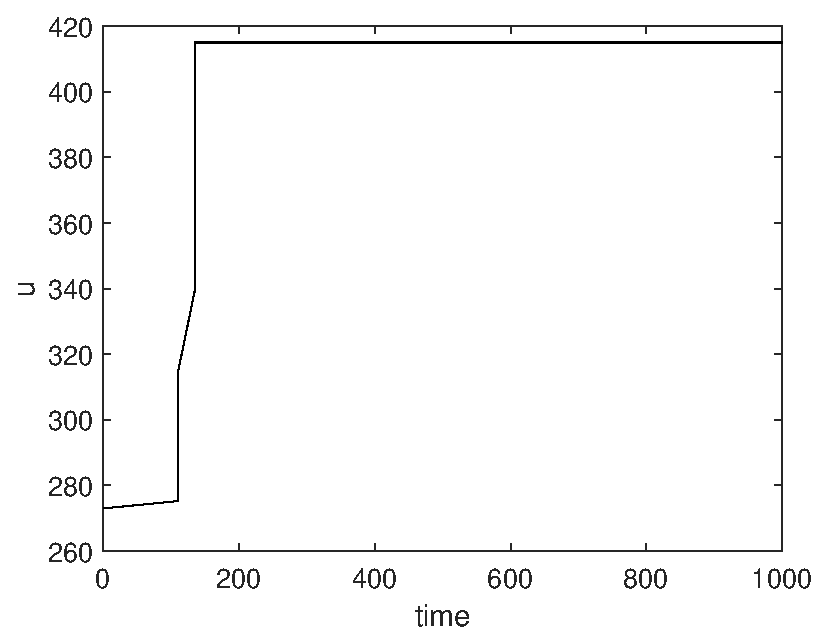
\includegraphics[width=0.99\textwidth]{examples/problem-denbigh_reactions/u_denbigh.eps}
		\caption[Tutorial example 6: control profile]{Control profile for
			Denbigh's system of reactions}\label{fig:probdenbigh_u} 
	\end{minipage}
	\begin{minipage}[t]{0.5\linewidth}
		\centering
		\includegraphics[width=0.99\textwidth]{examples/problem-denbigh_reactions/x_denbigh.eps}
		\caption[Tutorial example 6: state profiles]{State profiles for Denbigh's system of reactions}\label{fig:probdenbigh_x} 
	\end{minipage}
\end{figure}	
	
	
	
	
\end{document}	